\documentclass[a4paper, DIV=17]{scrartcl}

\usepackage{exsheets}
\usepackage{graphicx}
\usepackage{tikz}
\usetikzlibrary{arrows.meta}

\begin{document}

\section{Geometric optics}

\begin{question}
    A ray of light strikes a smooth and shiny surface as shown in the
    diagram below.  What is the angle of reflection?

    \begin{figure}[h]
	\begin{center}
	    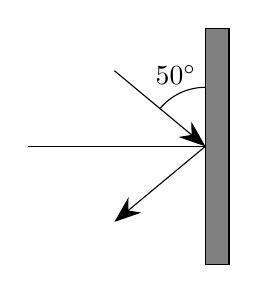
\begin{tikzpicture}[scale=1.5]
		\draw[fill=gray] (0, 1) -- (0, -1) -- (0.2, -1) -- (0.2, 1) -- cycle;
		\draw (-1.5, 0) -- (0, 0);
		\draw[-{Stealth[scale=2]}] (-0.77, 0.64) -- (0, 0);
		\draw[-{Stealth[scale=2]}] (0, 0) -- (-0.77, -0.64);
		\node (angle) at (-0.25, 0.6) {$50^\circ$};
		\draw (0, 0.5) arc[radius=0.5, start angle=90, end angle=140];
	\end{tikzpicture}
	\end{center}
    \end{figure}
\end{question}

\begin{solution}
    $40^\circ$
\end{solution}

\begin{question}
    A ray of light passes from air to water.  Given the options in the
    diagram below, which is the refracted ray?

    \begin{figure}[h]
	\begin{center}
	    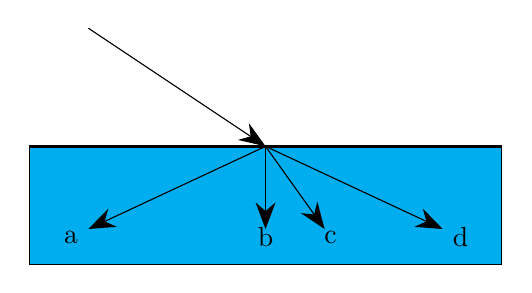
\begin{tikzpicture}[scale=1.5, >={Stealth[scale=2]}]
		\draw[fill=cyan] (-2, 0) -- (2, 0) -- (2, -1) -- (-2, -1) -- cycle;
		\draw[very thick] (-2, 0) -- (2, 0);
		\draw[->] (-1.5, 1) -- (0, 0);
		\draw[->] (0, 0) -- (-1.5, -0.7) node[pos=1.1] {a};
		\draw[->] (0, 0) -- (0, -0.7) node[pos=1.1] {b};
		\draw[->] (0, 0) -- (0.5, -0.7) node[pos=1.1] {c};
		\draw[->] (0, 0) -- (1.5, -0.7) node[pos=1.1] {d};
	\end{tikzpicture}
	\end{center}
    \end{figure}
\end{question}

\begin{solution}
    c
\end{solution}

\begin{question}[topic=geometric-optics]
    Using the equation defining the index of refraction, $n$, explain why
    the value of $n$ can never exceed the value 1.
\end{question}

\begin{question}
    The speed of light in a medium which is more optically dense than air is
    measured to be $2.012\times10^8$ m/s.  Calculate the index of
    refraction.
\end{question}

\begin{question}
Explain the meaning of the term \emph{normal incidence}.
\end{question}

\begin{question}
A light ray travelling in a low-density optical medium enters an optical
medium with a higher optical density.  Will the light ray refract
\emph{towards} or \emph{away from} the angle of normal incidence?

If the ray were travelling in the opposite direction (from a high-density
optical medium into a low-density optical medium), how will the light ray
refract with respect to the angle of normal incidence?
\end{question}

\begin{question}
\emph{Snell's law} describes the relationship between the angles of
incidence and refraction for a light ray crossing the boundary from one
optical medium to another:

\begin{equation}
    \frac{\sin \theta_1}{\sin \theta_2} = \frac{n_2}{n_1} = \frac{v_1}{v_2}
\end{equation}

\begin{figure}[h]
    \centerline{\includegraphics[height=6cm]{Snells_law2.png}}
    \caption{Snell's law; the ratio of the sines of the angle of incidence
    $\theta_1$ and the angle of refraction $\theta_2$ is equal to the ratio
    of indices of refraction $n_1$ and $n_2$, which is also equal to the
    ratio of the velocities of light in each medium $v_1$ and $v_2$.}
\end{figure}

    Considering a light ray travelling in air ($n \approx 1$) entering glass
    ($n = 1.52$) with an angle of incidence of $\theta_1 = 30^\circ$,
    what is the angle of refraction $\theta_2$?
\end{question}

\begin{question}
    Given Snell's law defined above, an approximate speed of light $c =
    3\times10^8$ m/s, and knowing the index of refraction in air, determine
    the speed of light in glass $v_2$ from the previous question.
\end{question}

\begin{question}
    We know that light rays leaving a high-density optical medium and
    travelling into a low-density optical medium refract \emph{away} from
    the angle of normal incidence.  This means that for rays leaving
    high-density optical media there will be an angle of incidence giving an
    angle of refraction equal to $90^\circ$ (i.e.~travelling parallel to the
    interface between the two optical media).  This angle is called the
    \emph{critical angle} and is often denoted by $\theta_c$.

\begin{figure}[h]
    \centerline{\includegraphics[width=\textwidth]{Refraction_reflection_critical_angle.png}}
    \caption{Reflection and refraction for a ray travelling from a
    more-dense optical medium into a less-dense optical medium.}
\end{figure}

    Using Snell's law, show that the critical angle can be written as:

    \begin{equation}
	\theta_c = \sin^{-1}\left(\frac{n_2}{n_1}\right)
    \end{equation}

\end{question}

\begin{question}
    Find the critical angle (in degrees) for a light ray travelling from
    water ($n = 1.33$) into air ($n = 1$).
\end{question}

\begin{solution}
    \begin{eqnarray}
	\theta_c &=& \sin^{-1}\left(\frac{n_2}{n_1}\right)\\
	&=& \sin^{-1}\left(\frac{1}{1.33}\right)\\
	&=& 0.8509\ \mathrm{radians}\\
	&=& 0.8509 \times \frac{180}{\pi}\ \mathrm{degrees}\\
	&=& 48.75^\circ
    \end{eqnarray}
\end{solution}

% \printsolutions

\end{document}
